\documentclass[12pt]{report}
\usepackage{geometry}
\usepackage{graphicx}
\usepackage{caption}
\usepackage{subcaption}
\graphicspath{{images/}}
\textheight 600pt
\textwidth 440pt
\bibliographystyle{ieeetran}
\setlength{\parskip}{1em}
\usepackage{array}
\usepackage{float}

\newcolumntype{C}[1]{>{\centering\arraybackslash}m{#1}}
\usepackage{etoolbox} % for "\patchcmd" macro
\makeatletter
% No extra space between chapter number and chapter header lines:
\patchcmd{\@makechapterhead} {\vskip 20}{\vskip 0} {}{}
% Reduce extra space between chapter header and section header lines by 50%:
\patchcmd{\@makechapterhead} {\vskip 40}{\vskip 20}{}{}
\patchcmd{\@makeschapterhead}{\vskip 40}{\vskip 20}{}{} % for unnumbered chapters
\makeatother


\begin{document}

\begin{titlepage}
    \begin{center}
        \Large
        \textbf{THESIS}\\
        \normalsize
        BACHELOR OF SCIENCE\\
        IN COMPUTER SCIENCE AND ENGINEERING \\
        \vspace{1.0cm}
        
        \textbf{AUTOMATIC DETECTION AND CLASSIFICATION OF DIABETIC RETINOPATHY STAGES IN RETINAL IMAGE}

        \vspace{2.0cm}
        
\includegraphics[width=0.3\textwidth]{iut}\\
        \vspace{1.0cm}
        ISLAMIC UNIVERSITY OF TECHNOLOGY\\
        GAZIPUR, BANGLADESH\\
        \vspace{3cm}
        
        
        MD. ABRAR LABIB\\
        \vspace{0.3cm}
        SAQUIB IRTIZA\\
        \vspace{0.5cm}
        2018\\
        \vspace{2.0cm}
        
        
       
        
        
    \end{center}
\end{titlepage}

\begin{titlepage}
    \begin{center}
        \vspace*{0.5cm}
        
        \textbf{AUTOMATIC DETECTION AND CLASSIFICATION OF DIABETIC RETINOPATHY STAGES IN RETINAL IMAGE}
        
        
        \normalsize
        \vspace{1.7cm}
        Authors:\\
        MD. ABRAR LABIB (ID: 144423)\\
        SAQUIB IRTIZA (ID: 144431)\\
        
        \vspace{1.0cm}
        A thesis submitted in partial fulfillment of the requirements for the degree of\\
        Bachelor of Science in Computer Science and Engineering\\
        \vspace{1.7cm}
        Supervisor:\\
        A.B.M. ASHIKUR RAHMAN\\
        Lecturer\\
        Department of CSE, IUT\\
        
        \vspace{1.7cm}
		
\includegraphics[width=0.2\textwidth]{iut}\\        
        \vspace{0.5cm}
        Islamic University of Technology\\
        Gazipur, Bangladesh\\
        
        
        
        
    \end{center}
\end{titlepage}

\newpage
\begin{titlepage}
\begin{center}
		\Large
		\textbf{Declaration}\\
\end{center}

\noindent This is to certify that the work presented in this thesis is the outcome of the analysis and investigation carried out by the candidates under the supervision of A.B.M. Ashikur Rahman in the Department of Computer Science and Engineering (CSE), at Islamic University of Technology (IUT), Gazipur, Bangladesh. It is also declared that neither this thesis nor any part of this thesis has been submitted anywhere else for any degree or diploma. Information derived from the published and unpublished work of others have been acknowledged in the text and a list of references is given.

\vspace{3.5cm}

\begin{table}[H]
\begin{center}
\begin{tabular}{C{7cm}C{8cm}}
\_\_\_\_\_\_\_\_\_\_\_\_\_\_\_\_\_\_\_\_\_\_\_\_\_\_\_\_\_\_\_\_\_&\_\_\_\_\_\_\_\_\_\_\_\_\_\_\_\_\_\_\_\_\_\_\_\_\_\_\_\_\_\_\_\_\_\\
\centering
(Signature of Candidate) & (Signature of Candidate)\\   
\centering
Md. Abrar Labib & Saquib Irtiza\\
\centering
Student ID: 144423 & Student ID: 144431\\
\centering
Academic Year: 2017-2018 & Academic Year: 2017-2018\\
\centering
November, 2018 & November, 2018\\
\end{tabular}
\end{center}
\end{table}

\vspace{3.0cm}


\begin{table}[H]
\begin{center}
\begin{tabular}{p{12cm}}
\centering 
\_\_\_\_\_\_\_\_\_\_\_\_\_\_\_\_\_\_\_\_\_\_\_\_\_\_\_\_\_\_\_\_\_\_\_\_\_\_\_\_\_\_\_\_\_\_\_\_\_\_\_\\
\centering 
(Signature of Supervisor)\\ 
\centering   
A.B.M Ashikur Rahman\\
\centering 
Lecturer\\
\centering 
Department of Computer Science and Engineering (CSE)\\
\centering 
Islamic University of Technology (IUT)\\
\centering 
November, 2018\\
\end{tabular}
\end{center}
\end{table}
\end{titlepage}


\Large
\begin{abstract}
\normalsize
\noindent This paper summarizes the different imaging techniques and methodologies used to perform classification of the different stages of a disease called diabetic retinopathy. In particular, it focuses on deep learning techniques to perform such detection in the fundus images of the patient's eye. Diabetic retinopathy is a progressive disease that causes the patient to lose eyesight if not diagnosed and treated at an early stage. Ophthalmologists usually diagnose the patient of this disease by screening the retinal fundus images to look for lesions. But the inaccuracy of such diagnosis together with the delay between diagnosis and treatment motivated researchers to automate this process of diagnosis. Using neural networks to train the system on a set of training images, it is possible to make systems that are more accurate and faster than human experts.  
\end{abstract}



\normalsize
\tableofcontents
\setlength{\parskip}{1em}

\chapter{Introduction}
\section{General Overview}
Visual perception is an integral part of human life. The eye is an organ that helps
humans in this perception by allowing them to interact with the world. It involves
sophisticated parts in the retinal region of the eye that reacts to the lighting condition
to which it is exposed to. Such parts include the light sensitive rods and cones that
send nervous impulses once light falls on it. These nervous impulses triggers the
brain and causes it to detect the object that the person sees.\\
\\Although this method of sensing is very crucial to the humans, it can be easily
impaired by various diseases, causing them to become blind in extreme cases. One
such disease is Diabetic Retinopathy (DR) that is very common in diabetic patients
and is one of the major reasons for such patients to lose their vision. It is also the
fastest growing cause of blindness in the world. But it is possible to eliminate the
risk of this disease if it is detected early and treated for accordingly.\\
\\The symptoms of this disease include growth of small legions or hemorrhages at
its initial stages. Ophthalmologists can detect such symptoms of the disease by
screening the fundus images of the eye. These are images of the retina taken through
the pupil. Any hemorrhages or legions detected in the image ensures that the patient
is positive of the disease. But detection of such lesions are difficult and often time
consuming since they are very small and complex structures. Hence researchers are
looking for ways to automate the detection procedure so that the ophthalmologists
can concentrate on treating the disease rather than detecting.
\newpage
\begin{figure}[h]
	\centering
	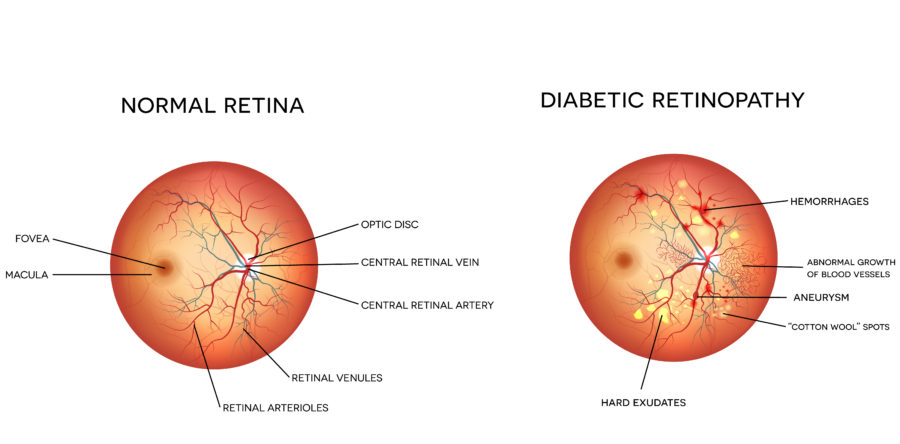
\includegraphics[width=1\textwidth]{fig1}
	\caption{Normal vs diseased retina}
	\label{fig1}
\end{figure}

\section{Motivation}
The increasing number of diabetic patients and the influx in blindness among these
patients caused by DR motivated us to work in this field. Also, the toll it takes on
the ophthalmologists to detect the complex symptoms, motivated us to automate
the system of detection so that they can concentrate more on treatment rather than
detection. The delay between the detection and treatment procedure also drove us
to work on this field because machines can detect the disease faster than humans.
\section{Purpose of this report}
This report initially elaborates on what the different stages of Diabetic Retinopathy
are and what are the symptoms of such stages. It also includes the motivation
that has driven us to work on this problem of automation. It then summarizes all
the related works that have been done on detection of Diabetic Retinopathy using
imaging techniques including works that have been done both with and without deep
learning techniques. Lastly we conclude the report with our proposed methods and
future works that can still be done in this field of research.
\chapter{Diabetic Retinopathy}
\section{Stages of Diabetic Retinopathy}
Diabetic Retinopathy (DR) occurs when tiny blood vessels in the retina are damaged
due to diabetes. These blood vessels leak blood or fluid forming lesions or hemorrhages that blur the vision of the patient. Each eye of a patient can be at different
stages of the disease. But for the sake of simplicity, we broadly categorize the the
disease into two categories:
\begin{itemize}
	\item[$\bullet$] Non-Proliferative Diabetic Retinopathy (NPDR)
	\item[$\bullet$] Proliferative Diabetic Retinopathy (PDR)
\end{itemize}
Non-Proliferative Diabetic Retinopathy is the initial stage of DR where the biological abnormalities starts growing. Depending on the extent of the growth, the stages can be further
categorized into mild and severe NPDR. If the disease still goes untreated, the final
stage of the disease, Proliferative DR is achieved.\\
\\Once PDR is reached, new blood vessels start growing at a very fast rate. The
tendency of the blood vessels to change and leak at the same time causes blindness
or complete loss of vision. Hence the level of severity of the disease can be classified
into 5 distinctive stages ranging from stage 0 to stage 4. Stage 0 is the safe state
whereas stage 4 is the most severe stage that usually leads to blindness. The stages
are:
\newpage
\begin{itemize}
	\item[$\bullet$] Stage 0: no DR
	\item[$\bullet$] Stage 1: mild DR
	\item[$\bullet$] Stage 2: moderate non-proliferative DR
	\item[$\bullet$] Stage 3: severe non-proliferative DR
	\item[$\bullet$] Stage 4: proliferative DR or Macular Edema (ME)
\end{itemize}

\begin{figure}[htpb]
	\centering
	\begin{subfigure}{.5\textwidth}
		\centering
		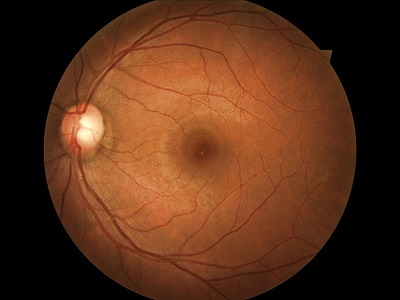
\includegraphics[width=.98\linewidth, height=.75\linewidth]{eye0}
		\caption{Stage 0}
		\label{eye0}
	\end{subfigure}%
	\begin{subfigure}{.5\textwidth}
		\centering
		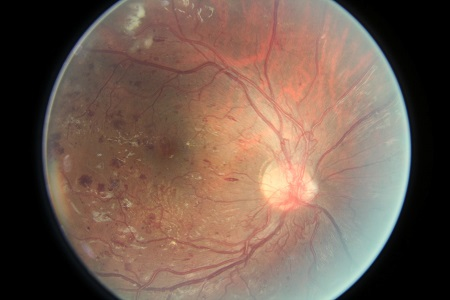
\includegraphics[width=.98\linewidth, height=.75\linewidth]{eye4}
		\caption{Stage 4}
		\label{eye4}
	\end{subfigure}
	\caption{Safe state versus severe state}
	\label{states}
\end{figure}
\section{Image Dataset Available}
In order to find a reliable model of neural network, we need a set of consistent high
quality images that can be used to train and compare the performance of the networks. Some available datasets are DIARET DB0 \cite{kauppi2006diaretdb0}, DIARET DB1 \cite{kalviainen2007diaretdb1}, MESSIDOR \cite{decenciere_feedback_2014}, and Kaggle \cite{kaggle_data}. Here we have listed the publicly available fundus image datasets
that are available:
\begin{itemize}
	\item[$\bullet$] Messidor-2 \cite{decenciere_feedback_2014}: Dataset of 1748 labelled color fundus images of 874 subjects with diabetes. Images of both the eyes of the subject are present in the dataset.
	\item[$\bullet$] Kaggle Dataset \cite{kaggle_data}: Dataset of 35126 labeled color fundus images of diabetic subjects. The dataset contains images of both the eyes of the patients. But the number of images in different classes are unbalanced and the images are of
	different aspect ratio. So, they need to be pre-processed before training.
\end{itemize}

\chapter{Literature Review}
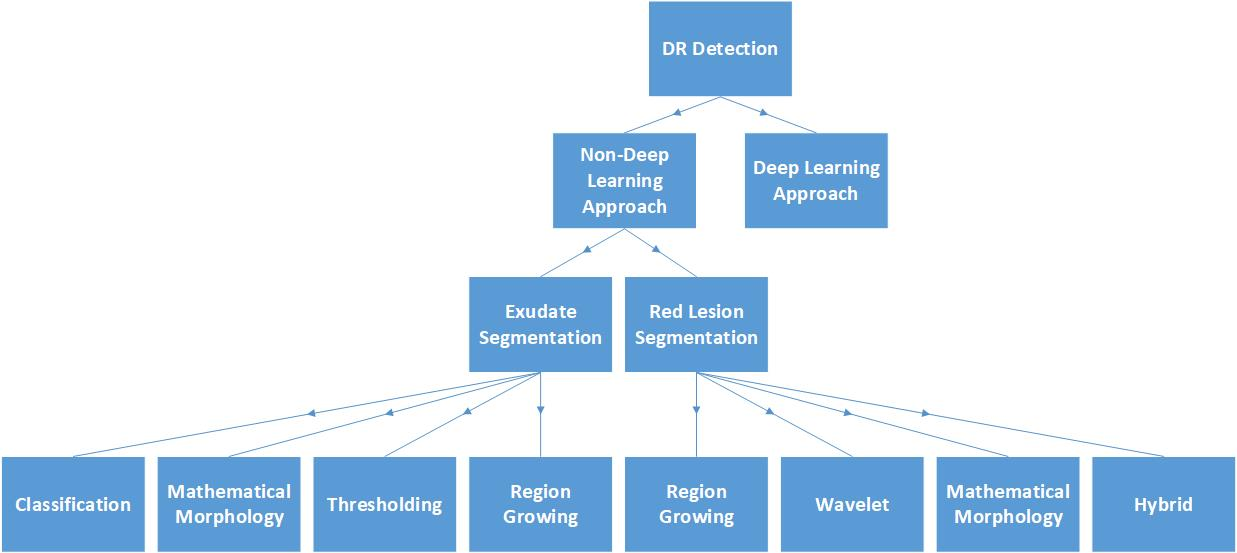
\includegraphics[width=1\textwidth]{Drawing1}

\section{Non Deep-Learning Methods}
Most non-deep learning approaches consist of several steps. Preprocessing steps such as contrast enhancement are usually carried out initially to lessen image variation by normalizing the original retinal image. Afterwards, irrelevant anatomical components such as the optic disk and vessels are removed. Finally, only the remaining pathological features of DR are retained for subsequent classification.

\noindent Non-deep learning methods from 2015 or earlier can be grouped into two types: exudate (EX) segmentation and red lesion (RL) segmentation.

\subsection{Exudate Segmentation}
EXs are lipoprotein intraretinal deposits due to vascular leakage. They appear in retinal images as yellowish lesions with well-defined edges. Their shape, size, brightness, and location vary among different patients. When clusters of EXs are located in the macular region, they are indicative of macular edema (ME), which is the main cause of visual loss in DR patients. For this reason, many researchers introduced the idea of a coordinate system based on the location of the fovea to determine DR grading. Different techniques have been proposed for EXs detection. They can be divided into four categories:

\subsubsection{■ Region Growing Method}
\subsubsection{o	Automated detection of diabetic retinopathy on digital fundus images (2008) \cite{sinthanayothin2002automated}.
}
\begin{itemize}
\item Authors: Sinthanayothin et al
\item Purpose: develop an automated screening system to analyse digital colour retinal images for important features of non-proliferative diabetic retinopathy (NPDR).
\item Method: High performance pre-processing of the colour images was performed. Previously described automated image analysis systems were used to detect major landmarks of the retinal image (optic disc, blood vessels and fovea). Recursive region growing segmentation algorithms combined with the use of a new technique, termed a ‘Moat Operator’, were used to automatically detect features of NPDR. These features included haemorrhages and microaneurysms (HMA), which were treated as one group, and hard exudates as another group.
\item Features:
\begin{itemize}
\item Hard exudates : identified as adjacent pixels with similar colour or grey level
\item HMA : sharpened using Moat Operator then identified by thresholding
\end{itemize}
\item Classifier: Multilayer perceptron neural network to identify blood vessels
\item Data: 112 digital fundus images of patients attending a DR screening service
\item Results: sensitivity and specificity for exudate detection were 88.5\% and 99.7\%
\end{itemize}

\subsubsection{■ Thresholding Method}
\subsubsection{o	Detection of exudates in retinal images using a pure splitting technique (2010) \cite{jaafar2010detection}.
}
\begin{itemize}
\item Authors: Jaafar et al
\item Method: an adaptive thresholding based on a novel algorithm for pure splitting of the image is proposed. A coarse segmentation based on the calculation of a local variation for all image pixels is used to outline the boundaries of all candidates which have clear borders. A morphological operation is used to refine the adaptive thresholding results based on the coarse segmentation results
\item Features:
\begin{itemize}
\item Exudates : local variation for each pixel of exudate region with clear margins
\item o	Non-exudates : discriminated using major axis length, minor axis length, area, solidity
\end{itemize}
\item Data: 50 abnormal images from DIARETDB0 database screening service
\item Results: 91.2\% sensitivity, 99.3\% specificity
\end{itemize}

\subsubsection{o	A novel automatic image processing algorithm for detection of hard exudates based on retinal image analysis (2008) \cite{sanchez2008novel}.
}
\begin{itemize}
\item Authors: Sanchez et al
\item Method: based on Fisher’s linear discriminant analysis and makes use of colour information to perform the classification of retinal exudates.
\item Features:
\begin{itemize}
\item Hard exudates : modified RGB model
\item Non-exudates : selecting pixels around optic disk depending on its area
\end{itemize}
\item Classifier: Fisher’s linear discriminant (FLD)
\item Data: 58 retinal images with variable colour, brightness, and quality
\item Results: sensitivity of 88\% using the lesion-based performance evaluation criterion, and accuracy of 100\% (sensitivity of 100\% and specificity of 100\%) image-based classification
\end{itemize}

\subsubsection{■ Mathematical Morpholopy Methods}
\subsubsection{o	Exudate detection in color retinal images for mass screening of diabetic retinopathy (2014). \cite{zhang2014exudate}}
\begin{itemize}
\item Authors: Zhang et al
\item Purpose: automatically detect normal exams in a tele-ophthalmology network, thus reducing the burden on the readers
\item Method: new preprocessing methods, which perform not only normalization and denoising tasks, but also detect reflections and artifacts in the image. A new candidates segmentation method, based on mathematical morphology. These candidates are characterized using classical features, but also novel contextual features. A random forest algorithm is used to detect the exudates among the candidates
\item Features:
\begin{itemize}
\item Contextual : distance between barycenter of candidate to nearest vessel, minimum distance of candidate to nearest vessel
\item Ultimate opening, a multi-scale morphological operator
\item Mean value of normalized saturation channel of each exudate candidate
\end{itemize}
\item Classifier: Random forest method
\item Data: A new clinical database, e-ophtha EX, containing precisely manually contoured exudates. It is very heterogeneous. It contains images gathered within the OPHDIAT telemedicine network for diabetic retinopathy screening
\item Results: AUC between 0.93 and 0.95
\end{itemize}

\subsubsection{o	Automatic detection of diabetic retinopathy exudates from non-dilated retinal images using mathematical morphology methods (2008). \cite{sopharak2008automatic}}
\begin{itemize}
\item Authors: Sopharak et al
\item Method: Preprocessing (RGB to HIS, median filter, contrast enhancement, optic disc elimination), exudates detection (closing, local variation, thresholding, morphological reconstruction)
\item Features:
\begin{itemize}
\item Exudate detection : size of structuring element in dilation, window size in local variation operator, threshold valued calculated using Otsu algorithm
\item Macular detection : Applying closing operator then thresholding
\end{itemize}
\item Data: All digital retinal images were taken from patients with nondilated pupils taken at Thammasat University Hospital
\item Results: Results: sensitivity and specificity are 80\% and 99.5\%
\end{itemize}

\subsubsection{■ Classification Method}
\subsubsection{o	A computational-intelligence-based approach for detection of exudates in diabetic retinopathy images (2009). \cite{osareh2009computational}}
\begin{itemize}
\item Authors: Osareh et al
\item Objective: Automated identification of exudate pathologies in retinopathy images based on computational intelligence techniques.
\item Method: The color retinal images are segmented using fuzzy c-means clustering following some preprocessing steps, i.e., color normalization and contrast enhancement. The entire segmented images establish a dataset of regions. To classify these segmented regions into exudates and nonexudates, a set of initial features such as color, size, edge strength, and texture are extracted. A geneticbased algorithm is used to rank the features and identify the subset that gives the best classification results. The selected feature vectors are then classified using a multilayer neural network classifier.
\item Features:
\begin{itemize}
\item Exudate discrimination : compactness of region, region size, region edge strength, mean Luv values inside and outside the region and Gabor filter response features
\end{itemize}
\item Classifier: three-layer perceptron NN with 65 node input
\item Data: large image dataset consisting of 300 manually labeled retinal images
\item Results: 96.0\% sensitivity, 94.6\% specificity
\end{itemize}

\subsubsection{o	Neural network based detection of hard exudates in retinal images (2009). \cite{garcia2009neural}}
\begin{itemize}
\item Authors: Garcia et al
\item Method: an algorithm which includes a neural network (NN) classifier. Three NN classifiers were investigated: multilayer perceptron (MLP), radial basis function (RBF) and support vector machine (SVM)
\item Features:
\begin{itemize}
\item Exudates : mean RGB values inside and outside the region and their standard deviations, region size, compactness and edge strength
\end{itemize}
\item Data: 117 images with variable colour, brightness, and quality. 50 of them (from DR patients) were used to train the NN classifiers and 67 (40 from DR patients and 27 from healthy retinas) to test
\item Results: Using a lesion-based criterion, a mean sensitivity (SEl) of 88.14\% and a mean positive predictive value (PPVl) of 80.72\% for MLP. With RBF, SEl = 88.49\% and PPVl = 77.41\%, while SEl = 87.61\% and PPVl = 83.51\% using SVM
\end{itemize}

\subsubsection{o    Automated detection of exudates for diabetic retinopathy screening (2007). \cite{fleming2007automated}}
\begin{itemize}
\item Authors: Fleming et al
\item Method: Candidate exudates were detected using a multi-scale morphological process. Based on local properties, the likelihoods of a candidate being a member of classes exudate, drusen or background were determined. This leads to a likelihood of the image containing exudates which can be thresholded to create a binary decision
\item Features:
\begin{itemize}
\item Exudate candidate : normalized luminosity and its standard deviation, normalized boundary gradient, candidate area, distance from nearest MA detected, and standardized colour features
\end{itemize}
\item Classifier: SVM having radial basis function kernel
\item Data: 13 219 images of which 300 contained exudates
\item Results: sensitivity 95.0\% and specificity 84.6\%
\end{itemize}

\subsubsection{o    Automated Detection and Differentiation of Drusen, Exudates, and Cotton-Wool Spots in Digital Color Fundus Photographs for Diabetic Retinopathy Diagnosis (2007). \cite{niemeijer2007automated}}
\begin{itemize}
\item Authors: Niemeijer et al
\item Purpose: To describe and evaluate a machine learning–based, automated system to detect exudates and cotton-wool spots in digital color fundus photographs and differentiate them from drusen, for early diagnosis of diabetic retinopathy
\item Method: : Each pixel was classified, resulting in a so-called lesion probability map that indicates the probability that a pixel is part of a bright lesion. Pixels with high probability were grouped into probable lesion pixel clusters. Based on cluster characteristics each probable lesion pixel cluster was assigned a probability indicating the likelihood that the pixel cluster was a true bright lesion. Each bright lesion cluster likely to be a bright lesion was classified as exudate, cotton-wool spot or drusen.
\item Features:
\begin{itemize}
\item True bright lesion detection : area, perimeter, compactness, length, width, mean gradient, mean of green channel pixels, mean CIE-LUV intensities, local pixel contrast, distance to closest red lesion
\end{itemize}
\item Classifiers: k-NN and a linear discriminant analysis classifier
\item Data: Three hundred retinal images from one eye of 300 patients with diabetes were selected from a diabetic retinopathy telediagnosis database (nonmydriatic camera, two-field photography): 100 with previously diagnosed bright lesions and 200 without
\item Results: The system achieved an area under the receiver operating characteristic (ROC) curve of 0.95 and sensitivity/specificity pairs of 0.95/0.88 for the detection of bright lesions of any type
\end{itemize}

\subsection{Red Lesion Segmentation}
MAs are small saccular bulges in the walls of retinal capillary vessels. In color fundus images, MAs appear like round red dots with a diameter ranging from 10 to 100 µm. MAs are difficult to distinguish from dot-HEMs, which are a little bigger. MAs are normally the first retinal lesions that appear in DR and their number has a direct relationship to DR severity. Several approaches have been proposed for MAs segmentation through color image analysis. The techniques for RL detection can be also divided into four categories:

\subsubsection{■ Region Growing Methods}
\subsubsection{o    Automated microaneurysm detection using local contrast normalization and local vessel detection (2006). \cite{fleming2006automated}}
\begin{itemize}
\item Authors: Fleming et al
\item Method: Various methods for contrast normalization are compared. Best results were obtained with a method that uses the watershed transform to derive a region that contains no vessels or other lesions. Dots within vessels are handled successfully using a local vessel detection technique
\item Features: number of peaks in smoothed energy function, major axis length, eccentricity of the elliptical cross section of the paraboloid, depth of the candidate, energy at the boundary
\item Classifier: k-NN with k = 15
\item Data: images acquired from diabetic patients attending the Grampian Diabetes Retinal Screening Programme 1441 images were graded by a clinician for the presence of MAs
\item Results: sensitivity 85.4\% and specificity 83.1\%
\end{itemize}

\subsubsection{■ Mathematical Morphology Methods}
\subsubsection{o   Automated microaneurysm detection method based on eigenvalue analysis using hessian matrix in retinal fundus images (2013). \cite{inoue2013automated}}
\begin{itemize}
\item Authors: Inoue et al
\item Method: After image preprocessing, the MA candidate regions were detected by eigenvalue analysis using the Hessian matrix in green-channeled retinal fundus images. Then, 126 features were calculated for each candidate region. By a threshold operation based on feature analysis, false positive candidates were removed. The candidate regions were then classified either as MA or false positive using artificial neural networks (ANN) based on principal component analysis (PCA). The 126 features were reduced to 25 components by PCA, and were then inputted to ANN
\item Features: based on pixel value, shape, texture analysis, reduced using principal component analysis (PCA)
\item Classifier: Classifier: artificial neural network (ANN)
\item Data: 25 retinal images from the retinopathy online challenge (ROC) database
\item Results: true positive rate was 73%, with eight false positives per image
\end{itemize}

\subsubsection{o  Automated detection of red lesions from digital colour fundus photographs (2011). \cite{jaafar2011automated}}
\begin{itemize}
\item Authors: Jaafar et al
\item Method: After pre-processing, a morphological technique was used to segment red lesion candidates from the background and other retinal structures. Then a rule-based classifier was used to discriminate actual red lesions from artifacts. A novel method for blood vessel detection is also proposed to refine the detection of red lesions
\item Features: aspect ratio, area, perimeter, circularity, eccentricity, mean intensity, inner standard deviation
\item Classifier: Rule-based classifier
\item Data: standarised test set of 219 images
\item Results: sensitivity of 89.7\% and a specificity of 98.6\% (at lesion level)
\end{itemize}

\subsubsection{o  Detection of microaneurysms using multi-scale correlation coefficients (2010). \cite{zhang2010detection}}
\begin{itemize}
\item Authors: Zhang et al
\item Method: a new approach based on multi-scale correlation filtering (MSCF) and dynamic thresholding is developed. This consists of two levels, microaneurysm candidate detection (coarse level) and true microaneurysm classification (fine level)
\item Features: area, perimeter, aspect ratio, circularity of the candidate, total, average and normalized intensities, compactness
\item Classifier: Discrimination table
\item Data: ROC (retinopathy on-line challenge) and DIARETDB1 (standard diabetic retinopathy database)
\item Results: 2nd rank in ROC competition
\end{itemize}


\subsubsection{o   Automatic detection of microaneurysms in color fundus images (2007). \cite{walter2007automatic}}
\begin{itemize}
\item Authors: Walter et al
\item Method: The first step consists in image enhancement, shade correction and image normalization of the green channel. The second step aims at detecting candidates, i.e. all patterns possibly corresponding to MA, which is achieved by diameter closing and an automatic threshold scheme. Then, features are extracted, which are used in the last step to automatically classify candidates into real MA and other objects; the classification relies on kernel density estimation with variable bandwidth
\item Features: no. of pixels in region, circularity, mean and maximal values of top-hat, dynamic (a classical morphological contrast measure), outer and inner grey level mean and standard deviation, grey level contrast, colour contrast
\item Classifier: KNN
\item Data: 21 annotated images Grampian Diabetes Retinal Screening Programme 1441 images were graded by a clinician for the presence of MAs
\item Results: sensitivity was 88.5\% at an average number of 2.13 false positives per image
\end{itemize}

\subsubsection{■ Wavelet-Based Method}
\subsubsection{o    Optimal wavelet transform for the detection of microaneurysms in retina photographs (2008). \cite{quellec2008optimal}}
\begin{itemize}
\item Authors: Quellec et al
\item Method: MAs are detected by locally matching a lesion template in subbands of wavelet transformed images. To improve the method performance, the best adapted wavelet within the lifting scheme framework is used. The optimization process is based on a genetic algorithm followed by Powell’s direction set descent
\item Data: 120 retinal images analyzed by an expert
\item Results: sensitivity of 89.62\%, positive predictive value of 89.50\%
\end{itemize}

\subsubsection{■ Hybrid Methods}
\subsubsection{o   Retinal Microaneurysm Detection Through Local Rotating Cross-Section Profile Analysis (2013). \cite{lazar2013retinal}}
\begin{itemize}
\item Authors: Lazar et al
\item Method: MA detection through the analysis of directional cross-section profiles centered on the local maximum pixels of the preprocessed image. Peak detection is applied on each profile, and a set of attributes regarding the size, height, and shape of the peak are calculated subsequently. The statistical measures of these attribute values as the orientation of the cross-section changes constitute the feature set that is used in a naïve Bayes classification to exclude spurious candidates. A formula for the final score of the remaining candidates is given, which can be thresholded further for a binary output
\item Features: increasing and decreasing ramp height, ramp slope, top and peak width, peak height
\item Classifier: Naïve Bayes classifier
\item Data: The ROC publicly available dataset consisting of 50 training and 50 test images
\item Results: overall score of 0.423, ranked 2nd in ROC competition
\end{itemize}

\subsubsection{o   Assessment of four neural network based classifiers to automatically detect red lesions in retinal images (2010). \cite{garcia2010assessment}}
\begin{itemize}
\item Authors: Garcia et al
\item Objective: detect red lesions (RLs), like haemorrhages and microaneurysms
\item Method: extracted a set of colour and shape features from image regions and performed feature selection using logistic regression. Four neural network (NN) based classifiers were subsequently used to obtain the final segmentation of RLs: multilayer perceptron (MLP), radial basis function (RBF), support vector machine (SVM) and a combination of these three NNs using a majority voting (MV) schema
\item Features: Region size, mean and standard deviation of RGB values in and around the region, compactness, edge strength, homogeneity, colour difference, circularity, eccentricity, aspect ratio
\item Classifiers: MLP, RBF, SVM
\item Data: 115 images divided into a training set of 50 images (with RLs) and a test set of 65 images (40 with RLs and 25 without RLs)
\item Results: best results were obtained for RBF. Using a lesion-based criterion, a mean sensitivity of 86.01\% and a mean positive predictive value of 51.99\% were obtained. With an image-based criterion, a mean sensitivity of 100\%, mean specificity of 56.00\%
\end{itemize}

\subsubsection{o   Mixture model-based clustering and logistic regression for automatic detection of microaneurysms in retinal images (2009). \cite{sanchez2009mixture}}
\begin{itemize}
\item Authors: Sanchez et al
\item Method: a statistical approach based on mixture model-based clustering and logistic regression. The innovative segmentation approach based on a statistical mixture model based clustering allows a robust separation of the foreground and background scenes and, specifically, a segmentation of MAS in a totally unsupervised manner
\item Features: based on shape, colour, brightness, contrast
\item Classifier: logistic regression classifier
\item Data: public database proposed by the Retinal Online Challenge
\item Results: overall score in the ROC competition of 0.332404
\end{itemize}

\subsubsection{o   Automated microaneurysm detection method based on double-ring filter and feature analysis in retinal fundus images (2009). \cite{mizutani2009automated}}
\begin{itemize}
\item Authors: Mizutani et al
\item Method: After image preprocessing, candidate regions for microaneurysms were detected using a double-ring filter. Any potential false positives located in the regions corresponding to blood vessels were removed by automatic extraction of blood vessels from the images. Twelve image features were determined, and the candidate lesions were classified into microaneurysms or false positives using the rule-based method and an artificial neural network
\item Features: area, circularity, length to width ratio, mean value of red, green and blue bits, contrast
\item Classifier: rule-based method and a three-layered feed forward ANN with back propagation algorithm
\item Data: Retinopathy Online Challenge (ROC) database (50 training cases, 50 test cases)
\item Results: sensitivity for detecting microaneurysms was 65\% at 27 false positives per image
\end{itemize}

\subsubsection{o   Automatic detection of red lesions in digital color fundus photographs (2005). \cite{niemeijer2005automatic}}
\begin{itemize}
\item Authors: Niemeijer et al
\item Method: a new red lesion candidate detection system based on pixel classification. Using this technique, vasculature and red lesions are separated from the background of the image. After removal of the connected vasculature the remaining objects are considered possible red lesions. An extensive number of new features are added to those proposed by Spencer–Frame. The detected candidate objects are classified using all features and a k-nearest neighbor classifier
\item Features: area, perimeter, aspect ratio, circularity, total, mean and normalized intensities in green plane and shade corrected image, compactness, mean and standard deviation of filter outputs
\item Classifier: kNN, linear discriminant, quadratic discriminant
\item Data: 100 images and was used to train and test composed of data taken from a screening program.
\item Results: sensitivity of 100\% at a specificity of 87\%
\end{itemize}

\section{Deep Learning Methods}
“Feature engineering,” involves computing explicit features specified by experts, resulting in algorithms designed to detect specific lesions or predicting the presence of any level of diabetic retinopathy. Deep learning is a machine learning technique that avoids such engineering by learning the most predictive features directly from the images given a large data set of labeled examples. This technique uses an optimization algorithm called back-propagation to indicate how a machine should change its internal parameters to best predict the desired output of an image. Some of the papers using deep learning algorithms to create models are given in the following section.

\subsection{Convolutional Neural Network}


A convolutional neural network (CNN) is a class of deep, feed-forward artificial neural networks. CNNs use a variation of multilayer perceptrons via backpropagation designed to require minimal preprocessing. CNNs use relatively little pre-processing compared to other image classification algorithms. This means that the network learns the filters that in traditional algorithms were hand-engineered. This independence from prior knowledge and human effort in feature design is a major advantage.




\subsubsection{■ Segmentation Using CNN}
\subsubsection{o   Development and Validation of a Deep Learning Algorithm for Detection of Diabetic Retinopathy in Retinal Fundus Photographs (2016). \cite{gulshan2016development}}
\begin{itemize}
\item Authors: Varun Gulshan et al
\item Objective: To apply deep learning to create an algorithm for automated detection of diabetic retinopathy and diabetic macular edema in retinal fundus photographs.
\item Method: CNN was implemented using Inception-v3 architecture proposed by Szegedy et al. The optimization algorithm used to train the network weights was a distributed stochastic gradient descent implementation by Dean et al. To speed up the training, batch normalization as well as preinitialization using weights from the same network trained to classify objects in the ImageNet data set were used. An ensemble of 10 networks trained on the same data was used, and the final prediction was computed by a linear average over the predictions of the ensemble.
\item Data: The EyePACS-1 data set consisted of 9963 images and Messidor-2 data set had 1748 images
\item Result: The performance of the algorithm at the high-sensitivity and high-specificity operating points are:
\begin{itemize}
\item High-sensitivity operating point: specificity was 84.0\% and sensitivity was 96.7\%.
\item High-specificity operating point: specificity was 93.8\% and sensitivity was 90.7\%
\item The area under the receiver operating characteristic curve was 97.4\%
\end{itemize}
\end{itemize}

\subsubsection{o   Improved Automated Detection of Diabetic Retinopathy on a Publicly Available Dataset Through Integration of Deep Learning (2016). \cite{abramoff2016improved}}
\begin{itemize}
\item Authors: Michael David Abramoff  et al
\item Objective: To compare performance of a deep-learning enhanced algorithm for automated detection of diabetic retinopathy.
\item Method: A hybrid device applies a set of CNN-based detectors to each of the images in the exam. These detectors are trained and optimized to detect normal retinal anatomy, such as optic disc and fovea, as well as the lesions characteristic for DR, such as hemorrhages, exudates, and neovascularization. They are inspired by Alexnet and the Oxford Visual Geometry Group network architectures. The analysis software provides four types of outputs:
\begin{itemize}
\item Negative: implying no or only mild DR present
\item rDR: implying rDR is present
\item vtDR: implying vtDR is present
\item Low exam quality: implying either protocol errors or low quality of the individual images.
\end{itemize}
If the index is above or equal to the vtDR threshold, a positive output for vtDR is returned. If the vtDR index is below this threshold, the rDR index is thresholded. If the rDR index is above or equal to this latter threshold a positive output for rDR is returned. If it is below the latter threshold an output of ‘‘negative’’ is returned. The device was never trained on any of the Messidor-2 images.
\item Data: 10,000 to 1,250,000 unique samples, depending on the lesion to be detected are used for training. Messidor-2 data consisting of 1748 images is used for validation.
\item Result: The device with CNN based detectors performed pretty good with results of:
\begin{itemize}
\item vtDR: 100\% sensitivity, 91\% specificity and 0.989 AUC.
\item rDR: 96.8\% sensitivity and 87.0\% specificity
\item The area under the receiver operating characteristic curve was 97.4\%
\end{itemize}
\end{itemize}

\subsubsection{o Fast convolutional neural network training using selective data sampling: Application to hemorrhage detection in color fundus images (2016). \cite{van2016fast}}
\begin{itemize}
\item Authors: van Grinsven et al
\item Objective: a method to improve and speed-up the CNN training for medical image analysis tasks by dynamically selecting misclassified negative samples during training
\item Method: A dynamic CNN training strategy where informative normal samples are dynamically selected at each training epoch from a large pool of medical images. A dynamic weight is assigned to each pixel in the negative training pool indicating its informativeness level. After each CNN training epoch, the weight of each negative training pixel is updated. This process is repeated until a stopping criterion is reached. The final trained CNN is used to classify each pixel in the test images, resulting in a pixel probability map for each test image
\item Network details: The CNN architecture used in this study consists of five convolutional layers followed by rectified linear units (ReLUs) and spatial max-pooling. The final layers of the network consist of a fully connected layer and a final softmax classification layer.
\item Data: Kaggle and Messidor databases
\item Result: A decreased training time from 170 epochs to 60 epochs with an increased performance – on par with two human experts – was achieved with areas under the receiver operating characteristics curve of 0.894 and 0.972 on two data sets. The SeS CNN statistically outperformed the NSeS CNN on an independent test set
\end{itemize}

\subsubsection{o Convolutional Neural Networks for Diabetic Retinopathy (2016). \cite{pratt2016convolutional}}
\begin{itemize}
\item Authors: Pratt et al
\item Objective: A network with CNN architecture and data augmentation which can identify the intricate features involved in the classification task such as micro-aneurysms, exudate and haemorrhages on the retina and consequently provide a diagnosis automatically and without user input
\item Method: Preprocessing tasks such as colour normalization and resizing were performed. The network was trained using stochastic gradient descent with Nestrov momentum. Afterwards, real-time dataaugmentation was used throughout training to improve the localisation ability of the network
\item Network details:  The network starts with convolution blocks with activation and then batch normalisation after each convolution layer. As the number of feature maps increases they move to one batch normalisation per block. All maxpooling is performed with kernel size 3x3 and 2x2 strides. After the final convolutional block the network is flattened to one dimension. To avoid overfitting they used weighted class weights relative to the amount of images in each class. Likewise, they performed dropout on dense layers, to reduce overfitting, until they reached the dense five node classification layer which uses a softmax activation function to predict our classification. The leaky rectified linear unit13 activation function was used, applied with a value of 0.01, to stop over reliance on certain nodes in the network. Similarly, in the convolution layers, L2 regularisation was used for weight and biases. The network was also initialized with Gaussian initialisation to reduce initial training time. The loss function used to optimise was the widely used categorical cross-entropy function.
\item Data: Kaggle databases
\item Result: a sensitivity of 95\% and an accuracy of 75\% on 5,000 validation images
\end{itemize}

\subsubsection{o Improved Microaneurysm Detection using Deep Neural Networks (2016). \cite{haloi2015improved}}
\begin{itemize}
\item Authors: Haloi et al
\item Objective: a novel microaneurysm (MA) detection for early diabetic retinopathy screening using color fundus images
\item Method: Each pixel of the image is classified as either MA or non-MA using a deep neural network with dropout training procedure using maxout activation function. No preprocessing step or manual feature extraction is required
\item Network details: three convolutional layers each followed by a max-pooling layer and one fully connected layer. And a softmax layer on the top of the network with two neurons for MA and non-MA probability values
\item Data: Retinopathy Online Challenge (ROC) and Diaretdb1v2 database
\item Result: accuracy of 95\% with sensitivity and specificity of 97\% and 94\% respectively on Messidor dataset
\end{itemize}

\subsubsection{o Automated Identification of Diabetic Retinopathy Using Deep Learning (2017). \cite{gargeya2017automated}}
\begin{itemize}
\item Authors: Gargeya et al
\item Objective: to develop a data-driven deep learning algorithm to automate DR screening
\item Network details: convolutional parameter layers learn iteratively filters that transform input images into hierarchical feature maps, learning discriminative features at varying spatial levels without the need for manually tuned parameters. each convolutional layer used batch normalization and the ReLU nonlinearity function to ensure smooth training and prevent overfitting, while using 2-class categorical cross-entropy loss for class discrimination
\item Data: Messidor 2 and E-Optha databases
\item Result: a 0.94 and 0.95 AUC score
\end{itemize}

\chapter{Proposed Method}
\vspace{5pt}
\section{Skeleton of Proposed Method}

\noindent Our proposed method starts by performing a series of preprocessing steps to remove the Optic Disc from the retinal image since it does not contribute to the disease. This involves morphological operations such as opening and closing and other image processing techniques. The functions of Matlab came in handy to perform these steps with minimum difficulty. 

\noindent We then divide our original dataset of images into two equally sized datasets containing approximately half the number of images as the original dataset. This was done in order to reduce the runtime of the overall neural network with minimal or no loss in data accuracy compared to the original dataset. Also, it ensured that almost all the images from the original dataset were used in the neural network for training.  

\vspace{13pt}



\noindent In the third step we create bottleneck features for our dataset, one for every image. Bottlenecks are the features that are made to train the last step of the pretrained model. It reduces the access time during the training period since it does not have to access mutiple layers of a model trained from scratch.

\noindent The bottlenecks are then used to train the already pretrained models using different network architectures to achieve a full model. Differences in learning rates and the number of epochs affect how fast the the models are formed. Once the models are created the validation datasets are used to check the validation accuracy of the trained model. Since we use multiple datasets to train the model, we get multiple accuracy results. These accuracy results are averaged in the final step of the proposed method. The time needed to train each model are timed to calculate the runtime of the proposed method.

\begin{figure}[h]
\centering
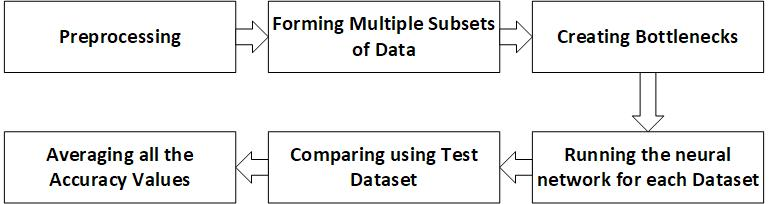
\includegraphics[width=1\textwidth]{Drawing2}
\caption{Skeleton of Method.}
\label{fig:test3}
\end{figure}

\section{Pre-Processing}

Optic disc (OD) has a specific set of characteristics that makes its removal fairly easy. It is usually circular in shape and of constant size, has high intensity and is found in the same exact location in every retinal image. Sometimes dark objects may appear in these optic disc regions which, if not removed beforehand, might contribute to the accuracy despite of having no genuine relation to the disease itself.

\noindent Since the position of the OD is fixed specifically in the middle third of the image, the following steps focus on that part of the retinal images particularly. We initially work on the red channel of the images since the intensity value of the OD is most distinct from the rest of the image in that color channel. The processing starts by resizing all the images to 600 by 800 pixels so that the complexity of the dataset is reduced and the results are obtained faster during training. 

\noindent The images are then passed through a median filter of size 11 by 11 pixels so that the finer blood vessels are filled up. The results are shown in Figure \ref{fig:sub2} . This filter does not blur out the border sharp edges such as the borders of OD or retina unlike other neighborhood averaging filters. It basically replaces the pixel at the center of the filter, $f_G(s,t) $, with pixel values of all its neighboring pixels as follows:

$$ 
f_{med}(x,y) = median_{(s,t)\epsilon W_{xy}}\{f_G(s,t)\}
$$

\noindent where W represents a neighborhood centered around location (x, y) in the image. On the resulting image we run a morphological top-hat transform so that it extracts small elements and details from given images. It involves performing a morphological opening operation on the input image based on a structuring element SE, and then subtracting the result from the original image itself as follows:

$$
T(f_{med}) = f_{med} - (f_{med}\circ SE)
$$

\noindent A disk structuring element of size 60 pixels is used for this operation making sure that the size of the structuring element is larger than the size of the OD. We then perform contrast stretching on the image so that it enhances the overall dynamic range of the image making the dark regions darker and bright regions brighter. A lower limit of 1\% and an upper limit of 80\% makes sure that the data is saturated at low and high intensities of image. The output image is shown in Figure \ref{fig:sub4}. 

\begin{figure}[h]
\centering
\begin{subfigure}{.5\textwidth}
  \centering
  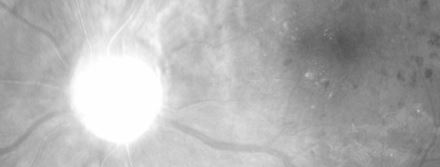
\includegraphics[width = 8cm, height =3cm]{Capture3}
  \caption{Red channel gray image.}
  \label{fig:sub1}
\end{subfigure}%
\begin{subfigure}{.5\textwidth}
  \centering
  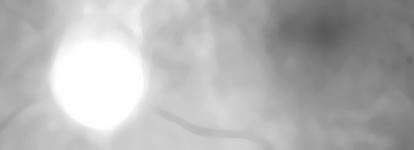
\includegraphics[width = 8cm, height =3cm]{Capture4}
  \caption{Output of using median filter.}
  \label{fig:sub2}
\end{subfigure}
\\
\begin{subfigure}{.5\textwidth}
  \centering
  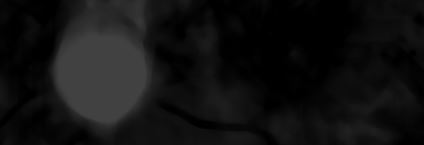
\includegraphics[width = 8cm, height =3cm]{Capture5}
  \caption{Output of using top-hat filter.}
  \label{fig:sub3}
\end{subfigure}%
\begin{subfigure}{.5\textwidth}
  \centering
  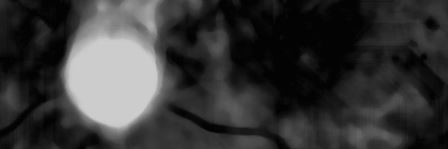
\includegraphics[width = 8cm, height =3cm]{Capture6}
  \caption{Contrast stretching.}
  \label{fig:sub4}
\end{subfigure}
\\
\begin{subfigure}{.5\textwidth}
  \centering
  
\includegraphics[width = 8cm, height =3cm]{Capture7}
  \caption{Binary image.}
  \label{fig:sub5}
\end{subfigure}%
\begin{subfigure}{.5\textwidth}
  \centering
  
\includegraphics[width = 8cm, height =3cm]{Capture8}
  \caption{Morphological opening and closing.}
  \label{fig:sub6}
\end{subfigure}
\caption{Presprocessing steps.}
\label{fig:test}
\end{figure}

\noindent A thresholding filter is then used to convert the image into a binary one. Because a threshold value of 0.7 is used, intensity values greater than this value are ceiled to one whereas all other values are considered zero. Figure \ref{fig:sub5} shows the result. Finally, a morphological opening is performed to further remove any small objects which are not part of the OD. This is followed by a closing operation using a disk structuring element of size 10 pixels to merge the adjacent objects together giving us an output as shown in Figure \ref{fig:sub6}.

\begin{figure}[h]
\centering
\begin{subfigure}{.5\textwidth}
  \centering
  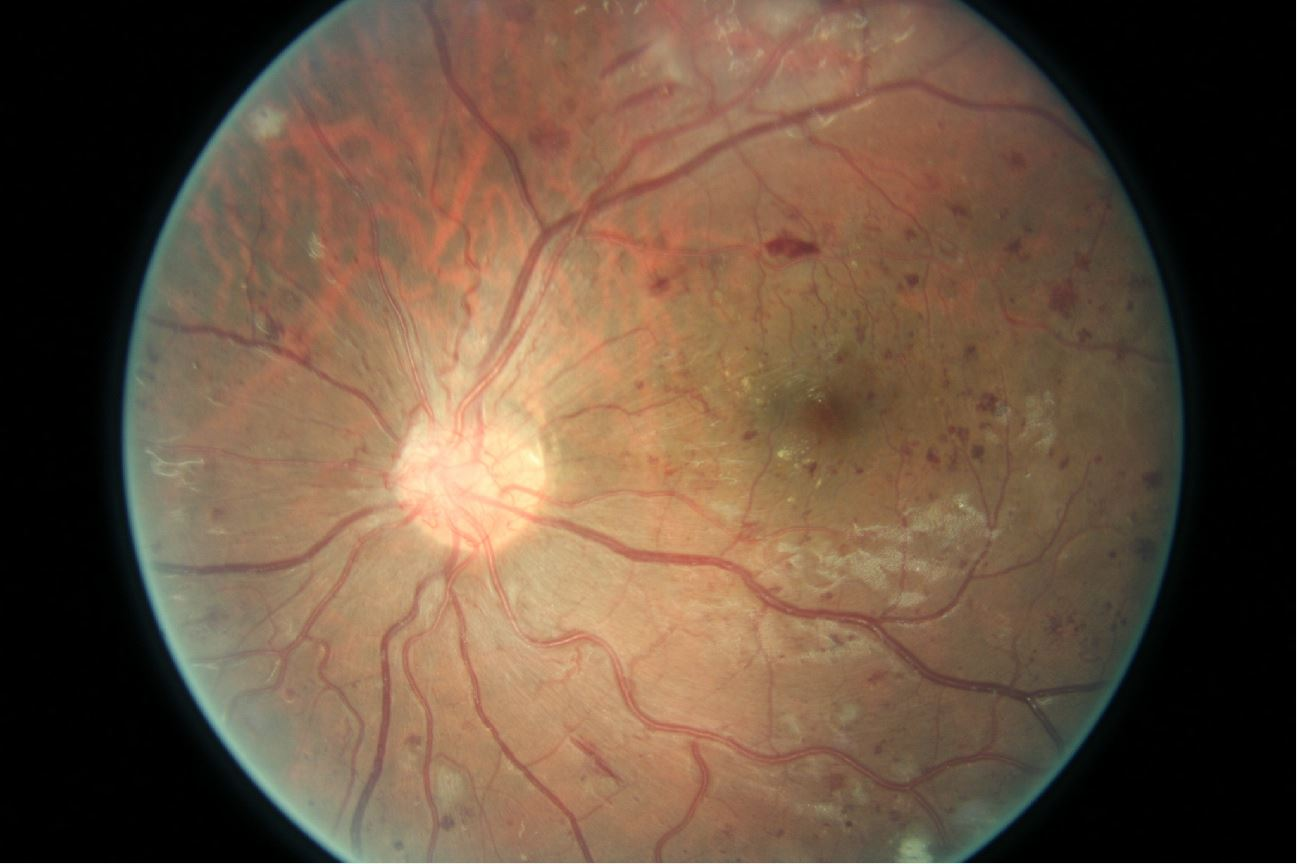
\includegraphics[width = 8cm, height =6cm]{Capture1}
  \caption{Original Image.}
  \label{fig:sub7}
\end{subfigure}%
\begin{subfigure}{.5\textwidth}
  \centering
  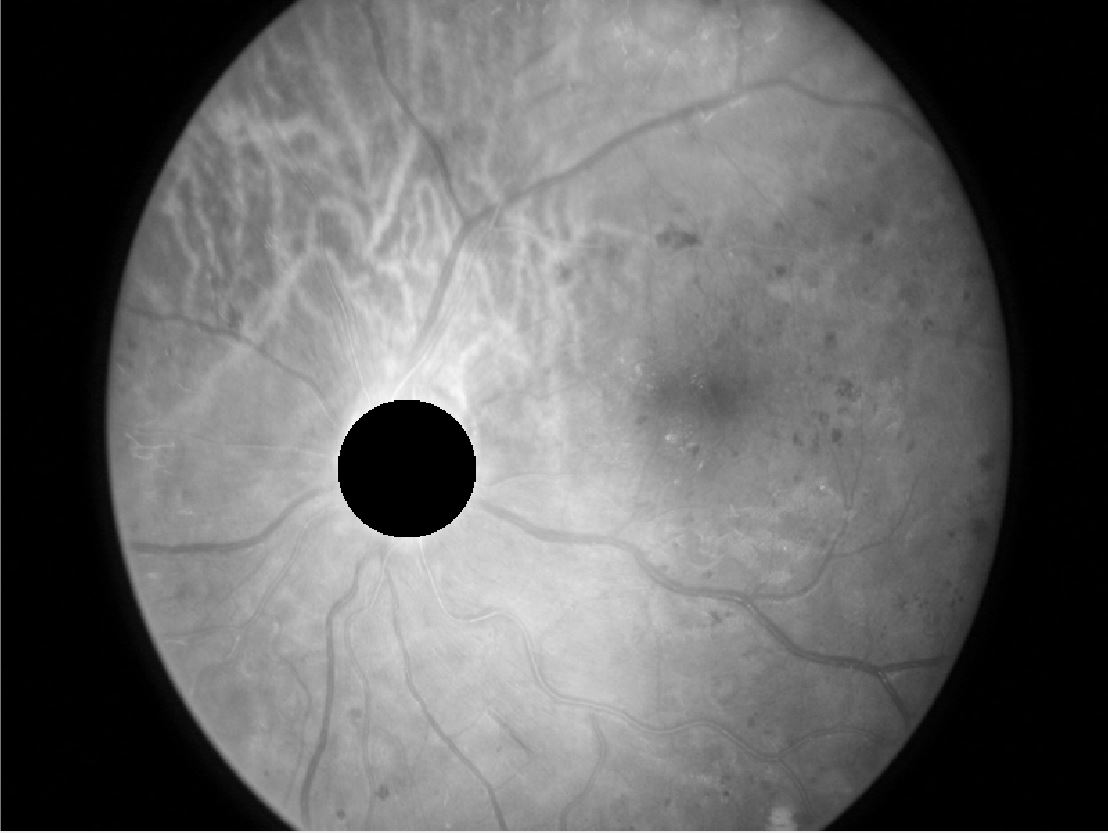
\includegraphics[width = 8cm, height =6cm]{Capture2}
  \caption{Image without the Optic disc.}
  \label{fig:sub8}
\end{subfigure}
\caption{Removal of Optic disc from the original image.}
\label{fig:test2}
\end{figure}

\noindent Since the output image now contains only the pixel values that contribute to the OD, we find the center of all the points that have a binary value of 1. Using this point as the center of a circle with a radius of 50 pixels, we remove any point from the original image that fall within this circle. This leaves us with an image that has its OD region blacked out as shown in Figure \ref{fig:test2}

\section{Preparation of Datasets}
The original dataset was divided into two smaller datasets of approximately half the number of images as the original dataset, each containing random images. This ensures that when we train the neural network with these datasets, majority of the images from the original dataset are used for training the network giving us a better accuracy. Also, training the network multiple times using these subsets of data helps improve the overall accuracy since the network gets to train more than once unlike the traditional method. 

\section{Transfer Learning}
Transfer learning is a research problem in machine learning that focuses on storing knowledge gained while solving one problem and applying it to a different but related problem. For example, considering model A's task is to identify 1000 kinds of objects like hats, cats, mats and we have such trained model at our hand, we want to create a model B to detect a cat/dog classifier. Even if we have a small dataset we can use the knowledge of model A during the training of model B and produce state of the art results. \cite{Transfer}

\noindent There are multiple reasons behind using this approach instead of taking the traditional training from scratch approach. Whenever we want to solve a unique problem using machine learning the chances are high that we might not find enough data for our model. Training with fewer data will result in not so good results. And even if we have large data there is a possibility of not having enough resources like GPU to obtain high-quality results. So transfer learning addresses these problems by already using the knowledge in the form of a pre-trained model which someone has created with large datasets, resources.

\begin{figure}[h]
\centering
\includegraphics[width=1\textwidth]{Pic1}
\caption{Transfer learning}
\label{fig:test4}
\end{figure}

\section{Architectures}
Different architectures for neural networks have been proposed by researchers over time that vary in its complexity and methodology. For our problem we use two different architectures namely Google's Inception V3 \cite{DBLP:journals/corr/SzegedyLJSRAEVR14} model and MobileNet \cite{DBLP:journals/corr/HowardZCKWWAA17} model to train our dataset of retinal images.

\subsection{Inception V3}

The inspiration comes from the idea that we need to decide whether we what a 3x3 or a 5x5 convolution at each layer of the model. Smaller convolutions recover local features whereas larger convolutions recover high abstracted features. So instead of deciding for ourselves as to what we want, we let the model decide for itself by finding all the convolutions at each layer and determining which convolution is most suitable at that layer. This operation is performed at each layer before it moves on. 

\begin{figure}[h]
\centering
\includegraphics[width=1\textwidth]{Pic2}
\caption{Inception module with dimension reduction.}
\label{fig:test5}
\end{figure}

\noindent The basic inception module shown in Figure \ref{fig:test5} gives us a brief demonstration of what operations are performed at each layer. It is evident that there are a large variety of convolutions being performed at each layer just as we mentioned earlier. The idea is that we don’t need to know ahead of time if it was better to do, for example, a 3×3 then a 5×5.  Instead, we let the model do all the convolutions and let it pick what's best.But there is also a max pooling layer alongside the convolutions. This was used just because historically, good networks had pooling. So to achieve greater accuracy, this operation was included. 

\begin{figure}[h]
\centering
\includegraphics[width=1\textwidth]{Pic3}
\caption{22 layers of Inception model.}
\label{fig:test6}
\end{figure}

\noindent But another major problem of this architecture is that the larger convolutions are more computationally expensive and takes a lot of time to compute. So in order to address the problem the paper suggests first doing a 1×1 convolution  reducing the dimensionality of its feature map, passing the resulting feature map through a relu, and then doing the larger convolution. The 1×1 convolution is key because it reduces the dimensionality of its feature map. The full architecture of the model is shown in Figure \ref{fig:test6}.

\subsection{MobileNet} 

MobileNet is an architecture which is more suitable for mobile and embedded based vision applications where there is lack of compute power.\cite{MobileNet} This architecture was proposed by Google. This architecture uses depthwise separable convolutions which significantly reduces the number of parameters when compared to the network with normal convolutions with the same depth in the networks. This results in light weight deep neural networks.The normal convolution is replaced by depthwise convolution followed by pointwise convolution which is called as depthwise separable convolution. 

\noindent In the normal convolution, if the input feature map is of $H_i,W_i,C_i$ dimension and we want $C_o$ feature maps with convolution kernel size $K$ then there are $C_o$ convolution kernels each with dimension $K,K,C_i$. This results in a feature map of $H_o,W_o,C_o$ dimension after convolution operation.

\noindent In the depthwise separable convolution, if the input feature map is of $H_i,W_i,C_i$ dimension and we want $C_o$ feature maps in the resulting feature map and the convolution kernel size is $K$ then there are $C_i$ convolution kernels, one for each input channel, with dimension $K,K,1$. This results in a feature map of $H_o,W_o,C_i$ after depthwise convolution. This is followed by pointwise convolution [1x1 convolution]. This convolution kernel is of dimension $1,1,C_i$ and there are $C_o$ different kernels which results in the feature map of $H_o,W_o,C_o$ dimension.

\noindent This results in the reduction of number of parameters significantly and thereby reduces the total number of floating point multiplication operations which is favorable in mobile and embedded vision applications with less compute power.By using depthwise separable convolutions, there is some sacrifice of accuracy for low complexity deep neural network.

\begin{figure}[h]
\centering
\includegraphics[width=0.7\textwidth]{Pic5}
\caption{MobileNet architecture.}
\label{fig:test7}
\end{figure}

\section{Averaging}

Since we used two different subsets of the same dataset containing random images, some of the images are common in both of them while others are not. This step helps in using a larger portion of the original dataset in training the neural network compared to only half the dataset. And because bottlenecks are needed to be formed only once for every image, the images that were common in both the datasets and have already been trained in the first dataset, do not need to be considered again when making bottlenecks for the second dataset. This reduces the combined runtime of the two training procedures compared to the runtime of a single traditional training procedure. Also, running the training steps twice for the two datsets, gives us two accuracy values, which upon averaging, gives us a more rigid accuracy value for the whole procedure. 


\chapter{Experimental Result and Performance Analysis}
\section{Dataset and Experimental Setup}
Implementations of diabetic retinopathy classification using CNN was attempted on a laptop computer having Core i7 2.6 GHz processor, 16 GB RAM and GTX 960M graphics card. These implementations were based on pretrained models developed by Google that were trained beforehand using approximately 14 million images of the ImageNet dataset. To train the final layer, we used our retinal image datasets of Messidor-2 and Kaggle. 

\noindent The code was implemented using python programming language on ubuntu operating system. Library functions such as OpenCV, Theano, Lasagna and Tensorflow were used. To carry out the preprocessing steps on the images, we used built-in functions of Matlab 2017 program such as top-hat transform and morphological opening and closing operations. The randomized subsets of data were also made using Matlab functions. All the operations in Matlab were performed in Windows 10 operating system and were later transferred to Ubuntu. 

\section{Performance Measurement}
In order to keep track of the performance of our proposed method compared to other methods, we used a set of metrics which are listed below. For a graphical representation we used Tensorboard which is a performance monitoring tool offered by Tensorflow. The metrics are:
\begin{itemize}
\item Training accuracy: Training accuracy gives us an estimate of what percentage of the training images the model could classify correctly. This is given by the number of  true positive images and the true negative images as a percentage of the total number of training images.

\item Validation accuracy: Similar to the training accuracy, we find the number of true positive and true negative images that the model managed to find correctly as a percentage of all the test images.But this time the accuracy is found for a different set of images that haven't been used in the training step before. This helps us understand how well our model performs for unknown images and whether our model is overfitted or not.

\item Cross Entropy: Cross-entropy is commonly used to quantify the difference between two probability distributions. The smaller the value of cross entropy the closer are the two probabilities. It is given by the equation:
$$
H(p,q)=-\sum_{x}p(x)log q(x)
$$

\item Runtime: Since our proposed method deals with ways to reduce the runtime of the training process without significantly losing accuracy, we need to keep track of the time it takes to execute the python scripts completely. The runtime includes time taken to create the unknown  bottlenecks and also the time necessary to run all the epochs of the training process.
\end{itemize}

\section{Comparative Analysis}
\subsection{Finding the right parameters}

\noindent For the first part of the experiment we used the two datasets without any preprocessing and varied the training iterations to see how the accuracy changed with change in epoch. Also all the images in the dataset were used for this experiment, a default learning rate of 0.01 was used and inception model was used as control. Notice that we haven't timed these experiments because we first wanted to find which dataset is more suitable to work on. The results are given in the table below:
\begin{table}[H]
\begin{center}
\begin{tabular}{ |p{5cm}|p{2cm}|p{2cm}|p{2cm}|p{2cm}| }
 \hline
 Dataset/Epochs & 500 & 1000 & 2000 & 4000\\ 
 \hline
 Kaggle & 55.7\% &  57.1\% &  58.8\% & 60.1\% \\  
 \hline
 Messidor-2 &  76.1\% &  77.7\% &  78.8\% &  81.9\%\\   
 \hline
\end{tabular}
\caption{Finding the appropriate dataset.}
\end{center}
\end{table}

\begin{figure}[H]
\centering
\begin{subfigure}{1\textwidth}
  \centering
  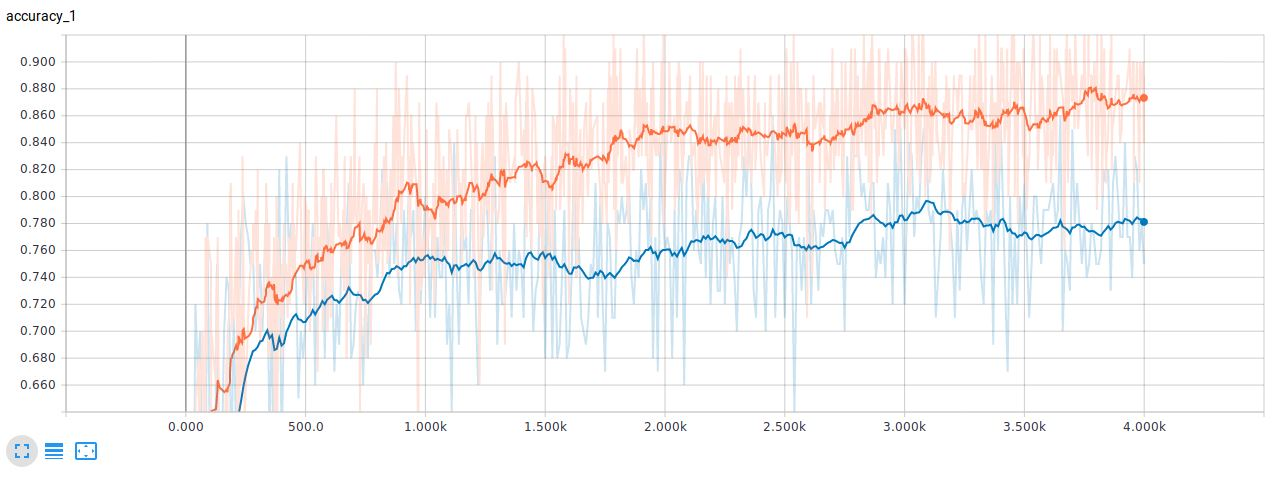
\includegraphics[width = 15cm, height =7cm]{Capture9}
  \caption{Variation of validation (blue) and training (orange) accuracy with every iteration.}
  \label{fig:sub9}
\end{subfigure}
\\
\begin{subfigure}{1\textwidth}
  \centering
  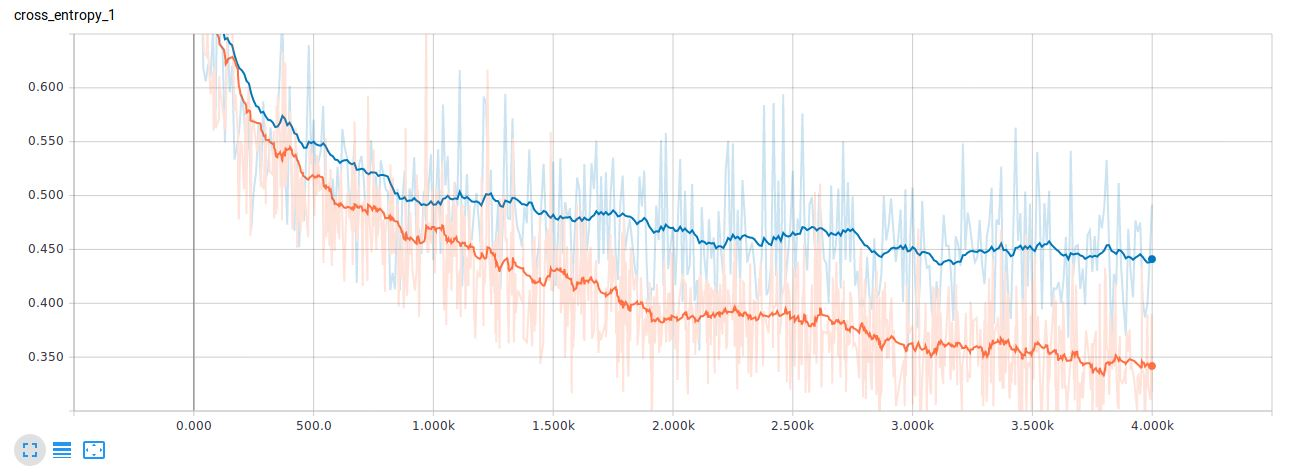
\includegraphics[width = 15cm, height =7cm]{Capture10}
  \caption{Variation of cross entropy with every iteration.}
  \label{fig:sub10}
\end{subfigure}
\caption{Graphical representation of performance metrics. }
\label{fig:test8}
\end{figure}

\noindent It is evident from the results that the dataset of Messidor-2 gives us more accurate results compared to Kaggle. This is because the images in Kaggle dataset are not standardized unlike Messidor-2 where all the images are centered, properly illuminated and of same size. Also with higher epochs, the accuracy values increase which indicates that the neural network learns better about the dataset with every epoch. The decrease in cross entropy with every epoch as shown in Figure \ref{fig:test8} also proves that the difference between the results and the expected output gets smaller with every iteration. 

\noindent We then move on to determine for which architecture of neural network we get the best accuracy results. Since we already found that Messidor-2 dataset gives us better accuracy, we keep that same for the experiments this time. We also use all the images in the dataset and a default learning rate of 0.01 as control values and find the results for different iterations. The results are as follows: 

\begin{table}[H]
\begin{center}
\begin{tabular}{ |p{5cm}|p{2cm}|p{2cm}|p{2cm}|p{2cm}| }
 \hline
 Architecture/Epochs & 500 & 1000 & 2000 & 4000\\ 
 \hline
 MobileNet &  65.4\% & 74.7\% &  78.7\% & 79.3\% \\  
 \hline
 Inception V3 & 76.1\% &  77.7\% &  78.8\% &  81.9\%\\   
 \hline
\end{tabular}
\caption{Finding the appropriate achitecture.}
\end{center}
\end{table}

\begin{figure}[h]
\centering
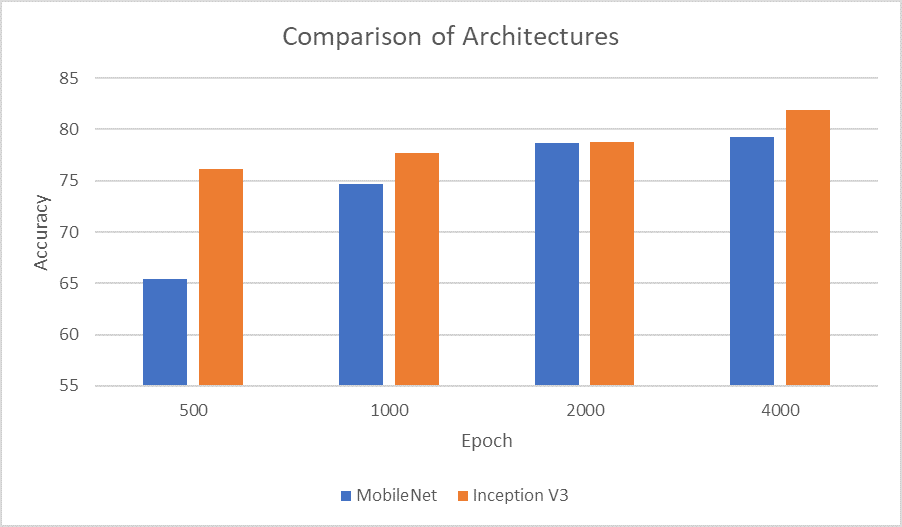
\includegraphics[width=1\textwidth]{Paint1}
\caption{Variation of accuracy for different architectures.}
\label{fig:test9}
\end{figure}

\noindent As Figure \ref{fig:test9} shows, results are indicative of the fact that Inception V3 is the better architecture here. So, we move on to find which learning rate is the most suitable for our dataset. Using the same dataset of Messidor-2 and architecture of Inception V3, we find which learning rate is the most appropriate. For all the experiments we maintain 500 epochs for faster runtimes assuming that the relative effect of learning rate still remain unaffected for this number of epochs. The results and a graphical representation are as follows:

\begin{table}[H]
\begin{center}
\begin{tabular}{ |p{5cm}|p{2cm}|p{2cm}|p{2cm}|p{2cm}| }
 \hline
 Learning rate & 0.005 & 0.01 & 0.1 & 0.5\\ 
 \hline
 Accuracy &   78.7\%&  76.1\% &   52.1\% &  42.0\%\\   
 \hline
\end{tabular}
\caption{Finding the best learning rate.}
\end{center}
\end{table}

\begin{figure}[h]
\centering
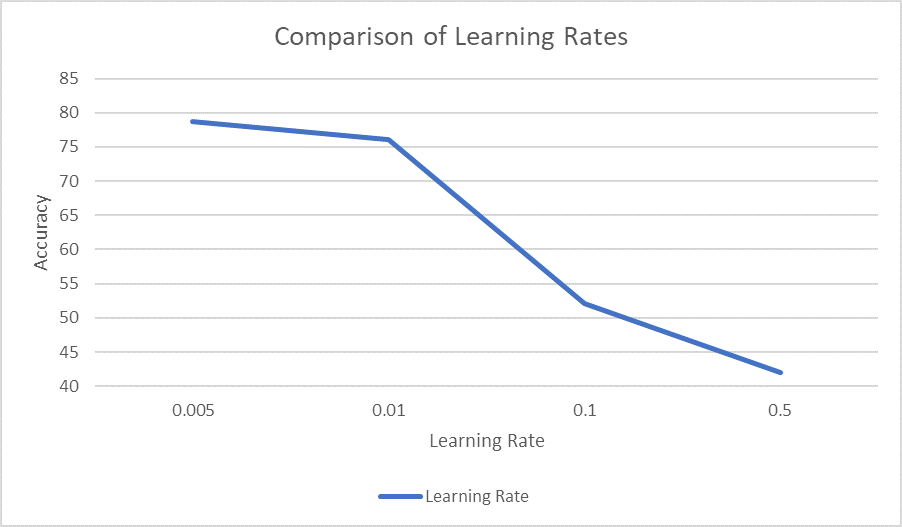
\includegraphics[width=1\textwidth]{Paint2}
\caption{Variation of accuracy for different learning rates.}
\label{fig:test10}
\end{figure}

\noindent The above set of experiments shows that for a small learning rate, like 0.005, the training takes longer, but the overall accuracy increases. Higher values of learning rate, like 1.0, trains faster, but typically reduces accuracy, or even makes training unstable. So for all the experiments following this we use a learning rate of 0.01 since it gives us a good balance between runtime and accuracy. Also to see how our preprocessing steps affect the accuracy, we run a series of experiments. The results are as follows:

\begin{table}[H]
\begin{center}
\begin{tabular}{ |p{5cm}|p{2cm}|p{2cm}|p{2cm}|p{2cm}| }
 \hline
 Dataset/Epochs & 500 & 1000 & 2000 & 4000\\ 
 \hline
 Normal &  76.1\% &  77.7\% &  78.8\% &  81.9\%\\ 
 \hline
 Preprocessed & 77.5\% &  79.5\% &  81.5\% & 83.4\%\\   
 \hline
\end{tabular}
\caption{Comparing the effects of preprocessing the images.}
\end{center}
\end{table}

\begin{figure}[h]
\centering
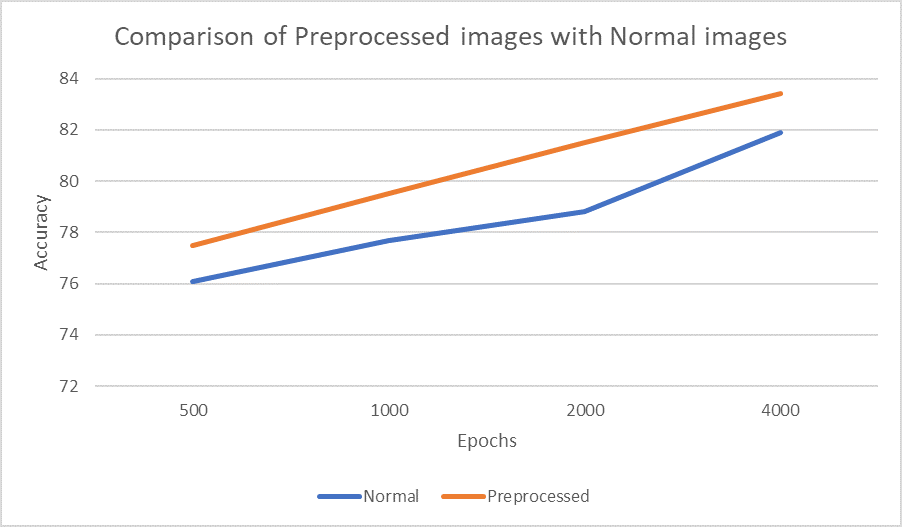
\includegraphics[width=1\textwidth]{Paint3}
\caption{Variation of accuracy for preprossed and normal images.}
\label{fig:test10}
\end{figure}


\noindent So, from the above set of experiments it is evident that in order to achieve optimal results, we should use Inception V3 architecture on Messidor-2 dataset and also ensure high number of epochs and a learning rate of 0.01 for the most optimal results. But despite of these optimal parameters, we could still have be far from optimizing the training process if it takes a long time. So, we address to this problem in the next section and propose a method to reduce the run-time.

\subsection{Reducing the run-time}

Once the appropriate parameters for the optimal results are obtained, we carry out our proposed method of reducing runtime to see how well it performs. The series of steps are as follows:

\begin{itemize}
\item Firstly we execute our set of preprocessing steps on Messidor-2 dataset. 
\item We then transfer the dataset to Ubuntu OS and divide the dataset into two subsets each containing approximately half the number of images as the original datset.
\item At this stage we initialize a timer to see how long it takes to get the results for the first subset of images.
\item We then begin the process of training our process which includes creating bottlenecks and finding the training and validation accuracy at each epoch. The parameters that we determined to be optimal are used for these steps.
\item Once all the epochs have been completed, we stop the timer and record the accuracy value and the runtime for the first subset.
\item We repeat the same set of steps for our second dataset and then find the total runtime and the average accuracy for the two sessions. 
\item To compare how well our method performed, we time a control session where we use the full dataset. The runtimes and the accuracy values that we get from the two methods are then compared. 

\end{itemize}

\noindent The results that we obtained are as follows:

\begin{table}[H]
\begin{center}
\begin{tabular}{ |p{5.5cm}|p{5cm}|p{5cm}| }
 \hline
 Method & Accuracy & Runtime\\ 
 \hline
 Traditional method &  77.7\% &  388.0s \\   
 \hline
 Proposed method (Attempt 1) &  $(72.7\%+78.0\%)/2 = 75.3\%$ &  $170.9s + 93.0s = 263.9 s$\\   
 \hline
 Proposed method (Attempt 2)&  $(70.2\%+73.4\%)/2 = 71.8\%$ &  $172.1s + 110.6s = 282.7s$\\   
 \hline
 Proposed method (Attempt 3)&  $(73.1\%+73.6\%)/2 = 73.3\%$ &  $158.7s + 104.2s = 262.9s$\\   
 \hline
\end{tabular}
\caption{Results of our proposed method.}
\end{center}
\end{table}

\noindent From the above set of results it is evident that the runtime for our proposed method reduces compared to traditional method but with a small trade-off of reduced accuracy. This process would be very useful in cases where the dataset is already very large and for any new images the accuracy does not increase by much. The ratio by which the reduction in runtime exceeds the reduction in accuracy in the first attempt is given by:
 
$$
\frac{\textbf{Runtime reduction}}{\textbf{Accuracy reduction}} = \frac{388-263.4}{77.7-75.3} = 52:1
$$

\noindent This reduction in runtime could be particularly useful in rural areas where doctors are not available for treatment and also powerful computers are not always at disposal for such computationally expensive processes. Although it is true that training would not be necessary after every patient's data is collected, it does need to be trained when a significant number of new images are collected waiting in line to be trained. In such cases if training a model from scratch takes days, patients would be deprived of prompt treatment. Hence for a small decrease in accuracy if there is an appreciable decrease in runtime, it could help training using low spec-ed computers in rural areas easier and in the process make way for more prompt treatment facilities.

\subsection{Prior study performance comparison}
The proposed method's performance was compared with previous methods in the field that have also been evaluated on the publicly available and independent Messidor-2 dataset. As stated before, our method achieved an accuracy of 75.3\% on this dataset, which is better than some of the previously published studies.\\
\noindent Both Sanchez et al. \cite{sanchez2011evaluation} and Seoud et al. \cite{seoud2016red} have proposed a computer-aided diagnosis system for diabetic retinopathy screening, comparable to the performance of human experts. Our method outperforms their approaches, both of which utilize non-deep learning methods.\\
A deep learning approach using a data-driven grading algorithm has been proposed by Gargeya et al. \cite{gargeya2017automated} has achieved impressive accuracy as well as reliability. Antal et al. \cite{antal2014ensemble} produce even more competitive results by using an ensemble of several retinal image processing algorithms that even outperform some of the deep learning approaches.\\
The previous two approaches perform significantly better than our proposed methods, but unfortunately none of the previous studies have published performance statistics that evaluate runtime. Since our intention is to implement the proposed method in remote or rural areas where quality medical screening is scarce, real-time runtime performance is absolutely crucial. As we have already demonstrated the reduction of run-time, we believe that the reasonable accuracy we have achieved is sufficient to make the proposed method a viable screening tool in deprived locales.

\begin{table}[H]
	\begin{center}
		\begin{tabular}{ |p{1.6cm}|p{2.35cm}|p{2.35cm}|p{2.35cm}|p{2.35cm}|p{2.35cm}| }
			\hline
			Methods & Sanchez et al. 2011 \cite{sanchez2011evaluation} & Seoud et al. 2016 \cite{seoud2016red} & Proposed Method & Gargeya et al. 2017 \cite{gargeya2017automated} & Antal et al. 2014 \cite{antal2014ensemble}\\ 
			\hline
			Accuracy &   59.0\%&  59.4\% &   75.3\% &  88.3\% & 90.8\%\\   
			\hline
		\end{tabular}
		\caption{Comparison of methods on the Messidor-2 dataset}
	\end{center}
\end{table}

\begin{figure}[h]
	\centering
	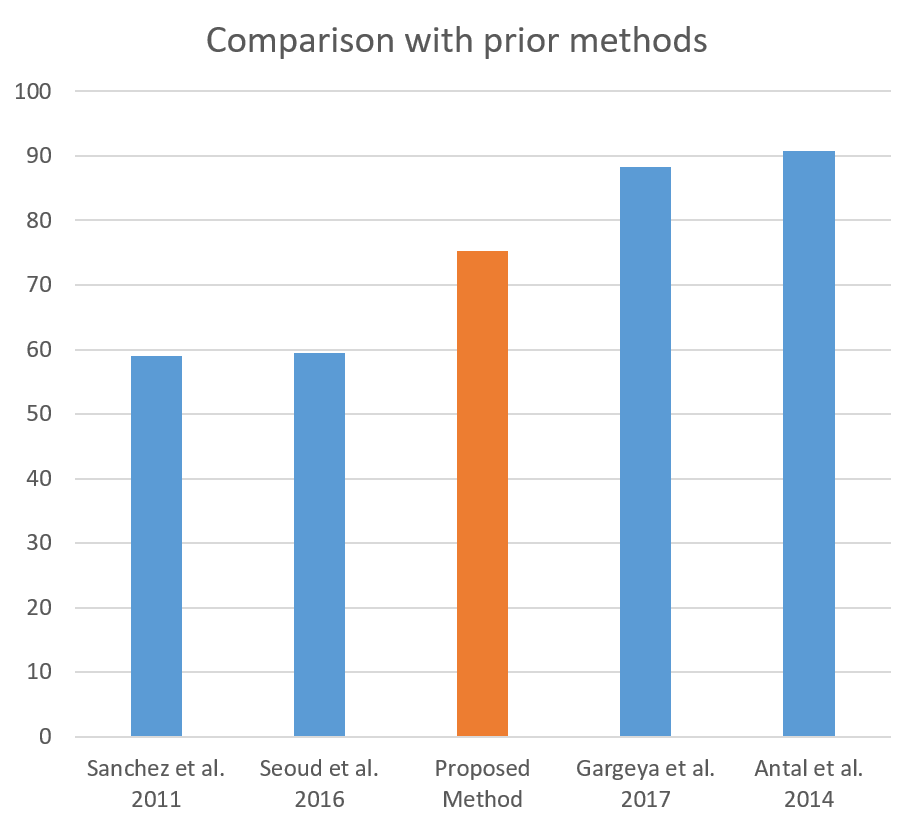
\includegraphics[width=1\textwidth]{comp}
	\caption{Model Comparison}
	\label{fig:test10}
\end{figure}





\chapter{Conclusion}
As discussed in this report, many works related to this field have already been done using deep learning and feature-based learning. But still, there is a scope to further enhance the techniques to improve efficiency and the complexity of the algorithms. Further research is necessary to determine the feasibility of applying this algorithm in the clinical setting and to determine whether use of the algorithm could lead to improved care and outcomes compared with current ophthalmologic assessment. And it is also very important that we address this problem at hand fast since the predicted numbers of people being infected by this disease are increasing everyday.

\section{Limitation}
Although we were able to reduce the runtime of the training process, we only used a small dataset to come to this conclusion. The Kaggle dataset is sufficiently large, but it is plagued by nagging problems such as varying resolutions and aspect ratios and different file types and illumination. Variation in illumination also prevented us from correctly removing the optical disc in pre-processing steps. Another persistent problem in all datasets is that the classes are unbalanced, with most of the images being in the negative class. This problem can be somewhat rectified by augmenting the dataset via rotation, flipping, etc. but that leads to overfitting of data. Since our method involves randomly segmenting the dataset, the ratio of run-time to accuracy is not going to be consistent. In order to justify the usefulness of our method, we also need to test our proposed method on larger datasets, to see if the run-time minimizations are substantial. The hardware on which we tested our proposed method also restricted us from training the network from scratch, which would have fetched better results. Another complication which may be relevant to our intention of building a screening tool for rural areas is that forming the dataset requires specialized equipment which may not be locally available.


\section{Future Works}
\begin{itemize}
\item Hardware permitting, we could try this approach with larger datasets or train the network from scratch
\item Try different neural network models such as RNN (Recurrent Neural Network), Inceptionv4, ResNet, VGG, etc.
\item Augment the dataset to balance the categories while also preventing overfitting
\item Perform segmentation to identify the regions of interest before feeding into the network
\item Use an ensemble method by using multiple networks and taking the best result
\item Instead of halving the dataset each time, we could divide into even smaller portions to observe which division produces the optimal run-time to accuracy ratio.
\item Use different preprocessing steps that increase the accuracy of the model such as:
\begin{itemize}
\item Images could be of different resolution. Enlarging all images to one common resolution might result in details to be lost. So we need to find optimum resolution for which the best accuracy is achieved.
\item There can be an unbalanced number of images in different classes. So we need to ensure consistency in the preprocessing step without overfitting.
\end{itemize}
\end{itemize}

\bibliography{Reference}




\end{document}